\documentclass[a4paper,12pt]{book}
\usepackage{graphicx}
\usepackage{pdfpages}

\begin{document}
	\tableofcontents
	\chapter{Input/Output and Forms Design}
	\section{Input Design}
	In an information system, input is the raw data that is processed to produce output. During the input design, the developers must consider the input devices such as PC, MICR, OMR, etc.
	
	input forms and screens have following properties 
		\begin{itemize}
	\item	It should serve specific purpose effectively such as storing, recording, and retrieving the information.
	\item	It ensures proper completion with accuracy.
	\item It should be easy to fill and straightforward.
	\item	It should focus on user’s attention, consistency, and simplicity.
		\end{itemize}
	
	
	\section{Objectives for Input Design}
	The objectives of input design are 
	\begin{itemize}
	\item 	To design data entry and input procedures
	\item 	To reduce input volume
	\item	To design source documents for data capture or devise other data capture methods
	\item 	To design input data records, data entry screens, user interface screens, etc.
	\item 	To use validation checks and develop effective input controls.
\end{itemize}
	
\section{Data Input Methods}
	Some of the popular data input methods are 
\begin{itemize}
	\item 	Batch input method (Offline data input method)
	\item 	Online data input method
	\item 	Computer readable forms
	\item 	Interactive data input
\end{itemize}
	
	
	
\section{Output Design}
	The design of output is the most important task of any system. During output design, developers identify the type of outputs needed, and consider the necessary output controls and prototype report layouts.
	
	
	\subsection{Objectives of Output Design}
	The objectives of input design are 
\begin{itemize}
	\item 	To develop output design that serves the intended purpose and eliminates the production of unwanted output.
	\item 	To develop the output design that meets the end users requirements.
	\item 	To deliver the appropriate quantity of output.
	\item 	To form the output in appropriate format and direct it to the right person.
	\item 	To make the output available on time for making good decisions.
\end{itemize}	
	\section{Forms Design}
	Both forms and reports are the product of input and output design and are business document consisting of specified data. The main difference is that forms provide fields for data input but reports are purely used for reading. For example, order forms, employment and credit application, etc.
	\section{Types of Forms}
	\subparagraph{Flat Forms}
	\begin{itemize}
	\item	It is a single copy form prepared manually or by a machine and printed on a paper. For additional copies of the original, carbon papers are inserted between copies.
	\item	It is a simplest and inexpensive form to design, print, and reproduce, which uses less volume.
	\end{itemize}
\subparagraph{Unit Set/Snap out Forms}
	\begin{itemize}
	\item	These are papers with one-time carbons interleaved into unit sets for either handwritten or machine use.
	\item	Carbons may be either blue or black, standard grade medium intensity. Generally, blue carbons are best for handwritten forms while black carbons are best for machine use.
	\end{itemize}
	\subparagraph{Continuous strip/Fanfold Forms}
	\begin{itemize}
	\item	These are multiple unit forms joined in a continuous strip with perforations between each pair of forms.
	\item	It is a less expensive method for large volume use.
	No Carbon Required (NCR) Paper
	\item	They use carbonless papers which have two chemical coatings (capsules), one on the face and the other on the back of a sheet of paper.
	\item	When pressure is applied, the two capsules interact and create an image.
	\end{itemize}
	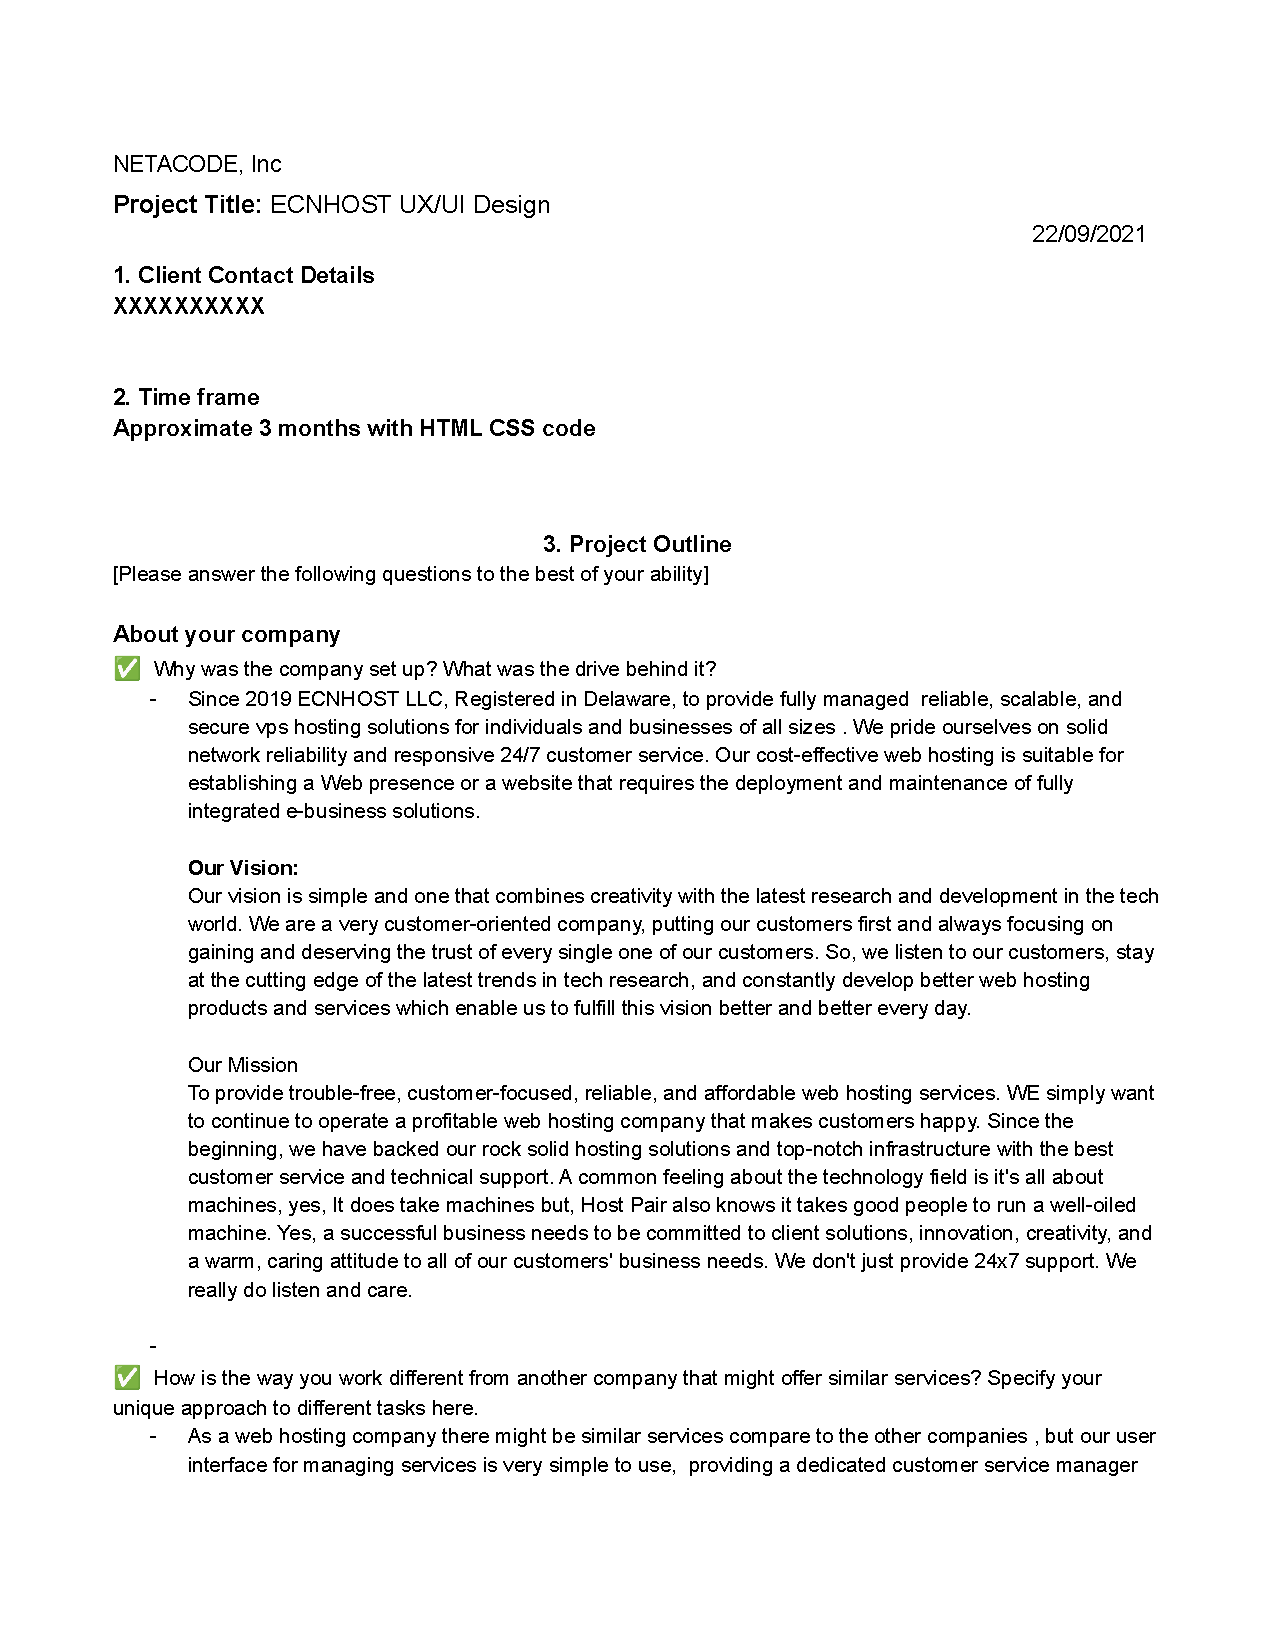
\includepdf[pages={1,2,3,4,5}] {mypdf.pdf}
	\section{Summary}
	With their consent, the information on the form above was gathered during the visit to Netacode Inc. and used in the report. The form is used by the organization to gather project requirements from clients. This form includes Client Contact Details, Project Time frame, Project Outline, Information on existing system, Website Architecture, Design Taste, Competition and Niche, Comment Section and a Sample Project output.

	\end{document}